\documentclass{article}
\usepackage[utf8]{inputenc} 

\usepackage{hyperref}

\usepackage[a4paper, total={6in, 8in}]{geometry}
\setlength{\parindent}{0em}

\usepackage{tikz}

\usepackage[french]{babel}  

\usepackage{amssymb}
\usepackage{amsmath}
\usepackage{amsthm}

\usepackage{float}

\usepackage{bigints}
\usepackage{relsize}

\usepackage{bbold}

\usepackage{cancel}

\usepackage{xcolor}

\makeatletter
\newcommand{\RemoveAlgoNumber}{\renewcommand{\fnum@algocf}{\AlCapSty{\AlCapFnt\algorithmcfname}}}
\newcommand{\RevertAlgoNumber}{\algocf@resetfnum}
\makeatother

\usepackage{minted}
\usepackage{newfloat}
\DeclareFloatingEnvironment{script} % new float <<<<


\newtheorem{theorem}{Théorème}
\newtheorem{contre-exemple}{Contre-exemple}
\newtheorem{corollary}{Corollaire}
\newtheorem{proposition}{Proposition}
\newtheorem{hyp}{Hypothèse}
\newtheorem{definition}{Définition}

\usepackage[ruled,vlined]{algorithm2e}
\usepackage{caption}

\newenvironment{fonction}[1][htb]
  {\renewcommand{\algorithmcfname}{Fonction}% Update algorithm name
   \begin{algorithm}[#1]%
  }{\end{algorithm}}

\definecolor{bg}{RGB}{22,43,58}


\title{$\chi^2$ et Mélanges Uniformes}
\author{Cyril THOMMERET \\ LPSM - Sorbonne Université \\ SAFRAN Aircraft Engines}
\date{\today}



\begin{document}
    \maketitle
    \tableofcontents
    \vspace*{1.2cm}
    Nous avions défini, pour une fonction $\varphi$ génératrice d'une divergence, le critère suivant:
    $$ m_{\pi,\theta}:\, x\in\mathrm{supp}\,g\, \longmapsto \int(\varphi^\prime\circ\dfrac{g}{g_{\pi,\theta}})(t)\cdot{}g(t)\mathrm{d}t - (\varphi^\#\circ\dfrac{g}{g_{\pi,\theta}})(x)$$
    où $\varphi^\prime$ est la dérivée de $\varphi$ et où $\varphi^\#\equiv{}\mathrm{id}\circ\varphi^\prime - \varphi$. \\

    \section{Le contexte dans le cas $\chi^2$}
    \subsection{Cas général}

    Du point de vue de la divergence du $\chi^2$, la fonction génératrice s'écrit: $\varphi_{\chi^2}(t) = \dfrac{\{t-1\}^2}{2}$ (avec $\mathrm{dom}\,\varphi_{\chi^2}=\mathbb{R}$).\\
    
    Nous avons,

    \begin{align*}
        \varphi_{\chi^2}^\prime(t) & = t - 1 \\
        \varphi_{\chi^2}^\#(t) = t\cdot\varphi_{\chi^2}^\prime(t) - \varphi_{\chi^2}(t) & = \dfrac{t^2-1}{2} \\
    \end{align*}

    Nous détaillons dans ce qui suit la forme du point de vue de la divergence du $\chi^2$, des différents quantités intervenant dans la considération de la résolution de nos tests pour une densité de mélange $g_{\pi,\theta}$ arbitaire (nous verrons ensuite le cas des mélanges uniformes.)

    % La fonction densité peut être plus précisément explicitée, 
    % $$
    % g_{\pi,\eta}(x)          =
    % \left\{
    %     \begin{array}{ll}
    %         (1-\pi)\cdot{}1 + \dfrac{\pi}{\eta} = 1 + \pi\cdot(\frac{1}{\eta}-1)  & \quad\mbox{si } x\in\overline{(0,\eta)} \\
    %         1-\pi                 & \quad\mbox{si } x\in(\eta,1] \\
    %         %0                   & \quad\mbox{sinon}
    %     \end{array}
    % \right. 
    % $$

    \subsubsection{Calcul du critère}

    D'après ce qui précède, pour toute fonction $g$ mesurable d'intégrale $1$, et pour tout $x\in\mathrm{supp}\,g$,

    \begin{align*}
        \int (\varphi'_{\chi^2}\circ\dfrac{g}{g_{\pi,\theta}})(t)\cdot{}g(t) \,\mathrm{d}t & = \int \big\{\dfrac{g(t)}{g_{\pi,\theta}(t)}-1\big\}\cdot{}g(t) \,\mathrm{d}t \\
                                                                                % & = \int \dfrac{(g(t))^2}{g_{\pi,\theta}(t)}\mathrm{d}t\, - \underset{=1\mbox{ si $g$ densité}}{\underbrace{\int g(t)\mathrm{d}t}}\\
                                                                                & = \int \dfrac{(g(t))^2}{g_{\pi,\theta}(t)}\mathrm{d}t\, - 1\\
        \mbox{et }\hspace*{1.2cm}(\varphi^\#_{\chi^2}\circ\dfrac{g}{g_{\pi,\theta}})(x) & =  \dfrac{1}{2}\cdot\Big\{ \Big(\dfrac{g(x)}{g_{\pi,\theta}(x)}\Big)^2 - 1 \Big\}                                                                     
    \end{align*}

    Nous pouvons dès lors donner, dans le cadre de la divergence du $\chi^2$, la forme générale (au sens où la densité de mélange n'a pas encore été spécifiée) du critère $m_{\pi,\theta}$:

    \begin{align*}
        m_{\pi,\theta}^{\chi^2}(x) :   &= \int(\varphi_{\chi^2}^\prime\circ\dfrac{g}{g_{\pi,\theta}})(t)g(t)\mathrm{d}t - (\varphi_{\chi^2}^\#\circ\dfrac{g}{g_{\pi,\theta}})(x) \qquad\mbox{(par définition)}\\
                            &= \int \dfrac{(g(t))^2}{g_{\pi,\theta}(t)}\mathrm{d}t\, - 1 -\dfrac{1}{2}\cdot\Big[ \Big(\dfrac{g(x)}{g_{\pi,\theta}(x)}\Big)^2 - 1\Big] \qquad \mbox{(par substitution)}
                            % &= \int \dfrac{(g(t))^2}{g_{\pi,\theta}(t)}\mathrm{d}t - \dfrac{1}{2}\cdot\Big\{ \Big(\dfrac{g(x)}{g_{\pi,\theta}(x)}\Big)^2 + 1 \Big\}
    \end{align*}
    \hspace{1.1cm}$\implies \fbox{$m_{\pi,\theta}^{\chi^2}(x) = \mathop{\mathlarger{\int}} \dfrac{(g(t))^2}{g_{\pi,\theta}(t)}\mathrm{d}t - \dfrac{1}{2}\cdot\Big[ \Big(\dfrac{g(x)}{g_{\pi,\theta}(x)}\Big)^2 + 1 \Big]$}$ \\
    % $$ \fbox{$m_{\pi,\theta}(x) =  \int \dfrac{(g(t))^2}{g_{\pi,\theta}(t)}\mathrm{d}t - \dfrac{1}{2}\cdot\Big\{ \Big(\dfrac{g(x)}{g_{\pi,\theta}(x)}\Big)^2 + 1 \Big\}$} $$

    Dans les applications, nous serons amener à considérer les deux premières dérivées (selon $\pi$ et $\theta$) du critère précédemment explicité. Nous procédons ici à leurs déterminations \footnote{Ici, seules les dérivées par rapport à $\pi$ sont calculs puisque nous nous consacrons au cas d'exemple où $\theta_1^\star$ est connu.}

    \subsubsection{Calculs des dérivées du critères}

    \subsubsection*{Calcul de $\partial_\pi\,m_{\pi,\theta}$}

    {\color{red} Sous réserve d'une inversion entre dérivation-intégrale}, nous obtenons:

    $$\partial_\pi\,m_{\pi,\theta}(x) = \int(g(t))^2\cdot\partial_\pi\,g_{\pi,\theta}^{-1}(t)\,\cdot\mathrm{d}t - \dfrac{1}{2}\cdot(g(x))^2\cdot\partial_\pi\,g_{\pi,\theta}^{-2}(x) $$

    Premièrement,
    \begin{align*}
        \partial_\pi\, g_{\pi,\theta}^{-1}(x)   & = -\dfrac{\partial_\pi\,g_{\pi,\theta}(x)}{(g_{\pi,\theta}(x))^2} \\
                                                & = \dfrac{f_1(x|\theta_1)-f_2(x|\theta_2)}{(g_{\pi,\theta}(x))^2}
    \end{align*}

    Deuxièment,
    % \begin{align*}
    %     \partial_\pi\,g_{\pi,\theta}^{-2}(x)  &= -\dfrac{\partial_\pi\,\big[(g_{\pi,\theta}(x))^2\big]}{\big[(g_{\pi,\theta}(x))^2\big]^2} \\
    %                                         &= -\dfrac{2\cdot\big\{f_2(x|\theta)-f_1(x)\big\}\cdot{}g_{\pi,\theta}(x)}{(g_{\pi,\theta}(x))^4} \\
    %                                         &= 2\cdot\dfrac{\big\{f_1(x)-f_2(x|\theta)\big\}}{(g_{\pi,\theta}(x))^3}
    % \end{align*}
    \begin{align*}
        \partial_\pi\,g_{\pi,\theta}^{-2}(x)  &= -2\cdot\dfrac{\partial_\pi\,g_{\pi,\theta}(x)}{(g_{\pi,\theta}(x))^3} \\
                                            &= 2\cdot\dfrac{\big\{f_1(x|\theta_1)-f_2(x|\theta_2)\big\}}{(g_{\pi,\theta}(x))^3}
    \end{align*}

    Nous avons donc, finalement,

    $$\fbox{$\partial_\pi\,m_{\pi,\theta}(x) = \mathop{\mathlarger{\int}}\, \big(f_1(t|\theta_1)-f_2(t|\theta_2)\big)\cdot\Big\{\dfrac{g(t)}{g_{\pi,\theta}(t)}\Big\}^2\cdot\mathrm{d}t - \big\{f_1(x|\theta_1)-f_2(x|\theta_2)\big\}\cdot\dfrac{(g(x))^2}{(g_{\pi,\theta}(x))^3}$} $$

    \subsubsection*{Calcul de $\partial^2_\pi\,m_{\pi,\theta}$}

    % Pour pouvoir calculer $\partial^2_\pi\,P_\mathbb{X}\,m_{\hat\pi,\theta}$, nous déterminons $\partial^2_\pi\,m_{\hat\pi,\theta}$. En effet,

    % \begin{align*}
    %     \partial^2_\pi\,P_\mathbb{X}\,m_{\hat\pi,\theta} &= \partial^2_\pi\,\sum_{i=1}^{i=n}\,m_{\hat\pi,\theta}(X_i) \\
    %     \implies \hspace*{2cm}&= \sum_{i=1}^{i=n}\partial^2_\pi\,m_{\hat\pi,\theta}(X_i)
    % \end{align*}
 
    Il vient, d'après le calcul précédent de $\partial_\pi\,m_{\pi,\theta}$, {\color{red} toujours sous résevre d'un théorème de dérivation sous le signe intégrale},
    $$\partial^2_\pi\,m_{\pi,\theta}(x) = \int\{f_1(t|\theta_1) - f_2(t|\theta_2)\}\cdot\{g(t)\}^2\cdot\partial_\pi{}g^{-2}_{\pi,\theta}(t)\cdot\mathrm{d}t - \{f_1(x|\theta_1) - f_2(x|\theta_2)\}\cdot{g(x)}^2\cdot\partial_\pi\,g^{-3}_{\pi,\theta}(x) $$ 

    En outre,
    \begin{align*}
        \partial_\pi\, g^{-3}_{\pi,\theta}(x) & = -3\cdot\dfrac{\partial_\pi\,g_{\pi,\theta}(x)}{\{g_{\pi,\theta}(x)\}^4} \\
        & = 3\cdot\dfrac{f_1(x|\theta_1)-f_2(x|\theta_2)}{\{g_{\pi,\theta}(x)\}^4}
    \end{align*}

    Par conséquent,
    $$ \fbox{$\partial^2_\pi\,m_{\pi,\theta}(x) = 2\cdot\mathop{\mathlarger{\int}}\dfrac{\big[\{f_1(t|\theta_1)-f_2(t|\theta_2)\}\cdot{}g(t)\big]^2}{\{g_{\pi,\theta}(t)\}^3}\cdot\mathrm{d}t - 3\cdot\dfrac{\big[\{f_1(x|\theta_1)-f_2(x|\theta_2)\}\cdot{}g(x)\big]^2}{\{g_{\pi,\theta}(x)\}^4}$} $$


    \subsection{Applications aux mélange de lois uniformes}

    Plus particulièrement, nous pouvons développer ces formules en l'appliquant au modèle de mélange uniforme, défini à travers la densité,\footnote{Rappelons ici que nous considérons un modèle de mélange à deux composantes où $\theta_1^\star$, le paramètre des données de la première composante $f_1$ est supposé connu. En outre, $\theta_2$ sera substitué à $\eta$. Ainsi, $\theta_2^\star$, le paramètre des données de la seconde composante sera noté $\eta^\star$.}

    $$ g_{\pi,\eta} \equiv (1-\pi)\cdot\mathbb{1}_{\overline{(0,1)}} + \dfrac{\pi}{\eta}\cdot\mathbb{1}_{\overline{(0,\eta)}} \qquad (\forall\pi\in\overline{(0,1)})(\forall\eta\in(0,1))$$
    Par convenance nous prenons, $g\equiv\mathbb{1}_{\mathrm{suppp}\,g_{\pi,\eta}}\,\big( \equiv \mathbb{1}_{[0,1]} \big)$. \\

    En vue de quantifier le test issu du résultat de notre théorème, nous souhaitons pouvoir appliquer numériquement l'algorithme suivant:

    \SetKw{Apriori}{Données a priori:}
    \begin{algorithm}[h!]
    \caption{Algorithme général: Test d'homogénéité}
        \Apriori $\phi$, $\{f_1\}$, $\{f_2\}$, $\theta_1^\star$ \\
        \vspace*{0.2cm}
        \textbf{Input:} $n$, $n_{exp}$, $\tilde{n}$, $\mathcal{D}(\Theta_2)$, $\tilde{\mathcal{D}}(\Theta_2)$, $p$ \\
        \begin{enumerate}
            \item Générer le plan d'échantillonnage $\mathbb{X}_{n_{exp},n} = 
            \begin{bmatrix}
                \mathbb{X}^{(1)} \\
                \mathbb{X}^{(2)} \\
                \ldots \\
                \mathbb{X}^{(n_{exp})}
            \end{bmatrix} =
            \begin{bmatrix}
                X_{1,1} & X_{1,2} & \ldots & X_{1,n} \\
                X_{2,1} & X_{2,2} & \ldots & X_{2,n} \\
                \vdots  & \vdots  & \ddots & \vdots  \\
                X_{n_{exp},1} & X_{n_{exp},2} & \ldots & X_{n_{exp},n}
            \end{bmatrix}$ 
            où $X_{i,j} \sim g_{\pi^\star,\theta^\star}$. \hfill \break       
            \item Générer le vecteur $(t_k)_{1\leq k\leq n_{exp}}$ où $t_k := \textrm{Max}_{\eta\in\mathcal{D}(\Theta_2)}\, s_k(\eta)$ avec $s_k(\eta) := s(\mathbb{X}^{(k)},\eta)$. \vspace*{0.2cm}
            \item Générer la matrice $[t_{k,\tilde{k}}]_{\substack{1\leq k\leq n_{exp} \\ 1\leq\tilde{k}\leq\tilde{n}}}$ où $t_{k,\tilde{k}}:=\mathrm{Max}_{\eta\in\tilde{\mathcal{D}}(\Theta_2)}\,Y_\eta(\mathbb{X}^{(k)})$
        \end{enumerate}
        \begin{flushright}
            avec $(Y_\eta(\mathbb{X}))_{\eta\in\tilde{\mathcal{D}}(\Theta_2)}\sim\mathcal{N}(0,\Sigma(\mathbb{X}))$ et $\Sigma(\mathbb{X}):=\Big[\dfrac{b(\mathbb{X,\eta,\eta^\prime})}{\sqrt{a(\mathbb{X},\eta)\cdot{}a(\mathbb{X},\eta^\prime)}}\Big]_{\eta,\eta^\prime\in\tilde{\mathcal{D}}(\Theta_2)}$
        \end{flushright}
        \begin{enumerate}
        \setcounter{enumi}{4}
            \item Calculer le vecteur des probabilités de rejet $r:=\dfrac{1}{n_{exp}}\cdot\sum_{k=1}^{n_{exp}}\mathbb{1}\{t_k\geq t_{k,(\lceil \tilde{n}\cdot (1-p) \rceil)}\}$
        \end{enumerate}
    \end{algorithm}
    avec,
    \begin{align*}
        \hat\pi(\mathbb{X},\eta)    & := \arg\max_\pi\,P_\mathbb{X}\,m_{\pi,\eta} \\
        a(\mathbb{X,\eta})          %&:= \dfrac{P_\mathbb{X}\,\Psi^2_{\hat\pi}}{H_n^2} \\
                                    & := P_\mathbb{X}\big\{ (\partial_\pi\,m_{\hat\pi,\eta})^2 \big\} \Big\backslash \big[ \partial^2_\pi\,P_\mathbb{X}\,m_{\hat\pi,\eta} \big]^2 \\
        s(\mathbb{X},\eta)          & := \sqrt{\dfrac{|\mathbb{X}|}{a(\mathbb{X},\eta)}}\cdot\hat\pi(\mathbb{X},\eta) \\
        \mbox{et, }\quad b_n(\eta,\eta') & := \dfrac{ P_\mathbb{X}\Big[ \partial_\pi\,m_{\hat\pi(\eta),\eta} \cdot \partial_\pi\,m_{\hat\pi(\eta'),\eta'}\Big]}{P_\mathbb{X}\Big[ \partial^2_{\pi\pi}\,mm_{\hat\pi(\eta),\eta}\Big] \cdot P_\mathbb{X}\Big[ \partial^2_{\pi\pi}\,m_{\hat\pi(\eta'),\eta'}\Big]}
    \end{align*}
    \vspace*{0.5cm}

    Notons que dans le cas de la divergence du $\chi^2$, l'identité de Fisher n'est pas vérifiée, nous ne pouvons donc pas simplifier les expressions des dérivées (comme c'était le cas dans le cas de la divergence de Kullback-Leibler \textit{modifiée}.) \\

    Compte tenu de la forme particulière de la densité de mélange, nous pouvons en revanche toujours tenter de donner des expressions explicites au critère, ainsi qu'à ces dérivées première et seconde, afin que ces derniers puissent être calculables numériquement. \\

    \subsubsection{Étude et calcul de $\hat\pi(\mathbb{X},\eta)$}

    Comme dans le cas de la divergence de Kullback-Leibler \textit{modifié}, la densité de mélanges de lois uniformes tels que nous les considérons nous permet d'expliciter un peu plus, les différentes quantités intervants. \\

    Rappelons la forme du criètre,

    $$m_{\pi,\theta}^{\chi^2}(x) = \int_{\mathrm{supp}\,g} \dfrac{(g(t))^2}{g_{\pi,\theta}(t)}\mathrm{d}t - \dfrac{1}{2}\cdot\Big[ \Big(\dfrac{g(x)}{g_{\pi,\theta}(x)}\Big)^2 + 1 \Big]$$
    \vspace*{0.5cm}

    Pour tout $\eta\in(0,1)$, par définition, nous avons que,
    $$
    g_{\pi,\eta}(x)          =
    \left\{
        \begin{array}{ll}
            (1-\pi)\cdot{}1 + \dfrac{\pi}{\eta} = 1 + \frac{1-\eta}{\eta}\cdot\pi  & \quad\mbox{si } x\in\overline{(0,\eta)} \\
            1-\pi                 & \quad\mbox{si } x\in(\eta,1] \\
            %0                   & \quad\mbox{sinon}
        \end{array}
    \right. 
    $$
    
    \vspace*{0.3cm}
    Ainsi, la partie intégrale du critère $\mathop{\mathlarger{\int}} \dfrac{(g(t))^2}{g_{\pi,\theta}(t)}\mathrm{d}t$ devient $\mathop{\mathlarger{\int}}_0^\eta\, \dfrac{\mathrm{d}t}{1+\frac{1-\eta}{\eta}\cdot\pi} + \mathop{\mathlarger{\int}}_\eta^1\dfrac{\mathrm{d}t}{1-\pi}$ qui est \\ égal à $\dfrac{\eta}{1+\frac{1-\eta}{\eta}\cdot\pi} + \dfrac{1-\eta}{1-\pi}$. \\

    \vspace*{0.3cm}
    D'autre part, $\big\{ \dfrac{g(x)}{g_{\pi,\eta}(x)} \big\}^2$ prend la forme $\dfrac{1}{\big(\,1+\frac{1-\eta}{\eta}\cdot\pi\,\big)^2}\times\mathbb{1}_{\overline{(0,\eta)}}(x) + \dfrac{1}{\big(\,1-\pi\,\big)^2}\times\mathbb{1}_{(\eta,1]}(x)$. \\

    \vspace*{0.5cm}
    Par conséquent, dans le cas des mélanges uniformes tels que considérés, le critère s'écrit:

    $$ \fbox{$m_{\pi,\eta}(x) = \dfrac{\eta}{1+\frac{1-\eta}{\eta}\cdot\pi} + \dfrac{1-\eta}{1-\pi} - \dfrac{1}{2}\cdot\Big[\, \dfrac{\mathbb{1}_{\overline{(0,\eta)}}(x)}{\big(\,1+\frac{1-\eta}{\eta}\cdot\pi\,\big)^2} + \dfrac{\mathbb{1}_{(\eta,1]}(x)}{\big(\,1-\pi\,\big)^2} + 1 \,\Big]$}$$

    \vspace*{0.5cm}
    Soit $\mathbb{X}(\omega)=\mathbf{x}$ un échanillon de données. Il vient immédiatemment que,
    \vspace*{0.2cm}
    $$ \fbox{$P_\mathbb{X}\,m_{\pi,\eta} = \dfrac{\eta}{1+\frac{1-\eta}{\eta}\cdot\pi} + \dfrac{1-\eta}{1-\pi} - \dfrac{1}{2}\cdot\Big[\, \dfrac{p_-}{\big(\,1+\frac{1-\eta}{\eta}\cdot\pi\,\big)^2} + \dfrac{p_+}{\big(\,1-\pi\,\big)^2} + 1 \,\Big]$} $$
    
    \vspace*{0.3cm}
    avec $p_-$ (respectivement $p_+$) la proportion des données inférieures (respectivement supérieures) à $\eta$.\\

    Ainsi, la fonction à qui $\pi$ associe $P_\mathbb{X}\,m_{\pi,\eta}$, est continue sur tout compact $\overline{(0,\alpha)}$ avec $\alpha<1$. Nous pouvons donc dire que dès lors que $\pi\neq{}1$, la fonction atteint ses bornes, et donc que l'argument du maximum $\hat\pi$ existe. \\

    En outre, nous constatons par les graphes suivants que la fonction dont nous cherchons un maximum présente un aspect convexe, et cela pour différente valeur de $\eta$. \\

    \begin{figure}[H]
        \centering
        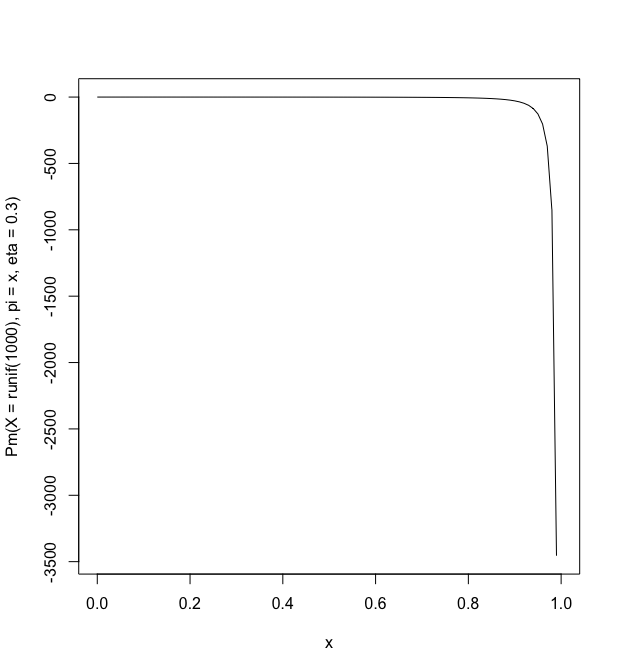
\includegraphics[scale=0.5]{img/Pm_1.png}
        \caption{Graphe de la fonction $\pi\mapsto{}P_\mathbb{X}\,m_{\pi,\eta}$ pour un échantillon de loi uniforme sur $\overline{(0,1)}$ de taille $10^3$ avec $\eta^\star=\eta=0.3$ ($\pi^\star=0$).}
    \end{figure}

    \begin{figure}[H]
        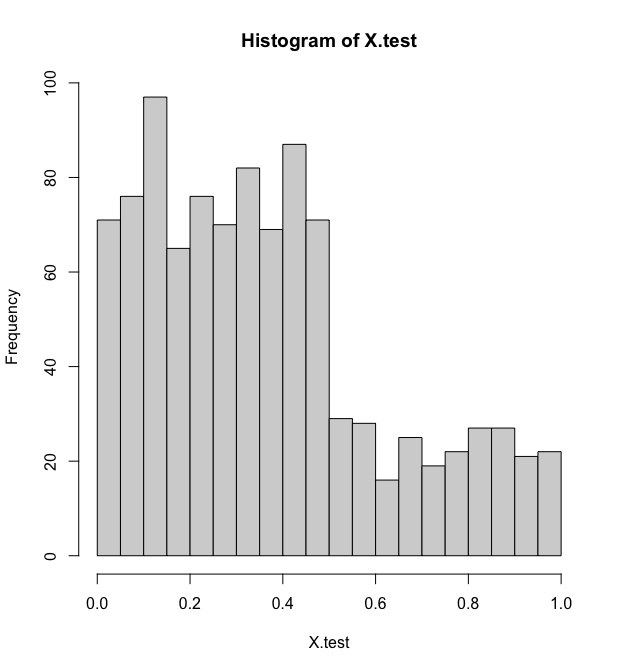
\includegraphics[width=0.5\textwidth]{img/hist_1.png}
        \hspace{\fill}
        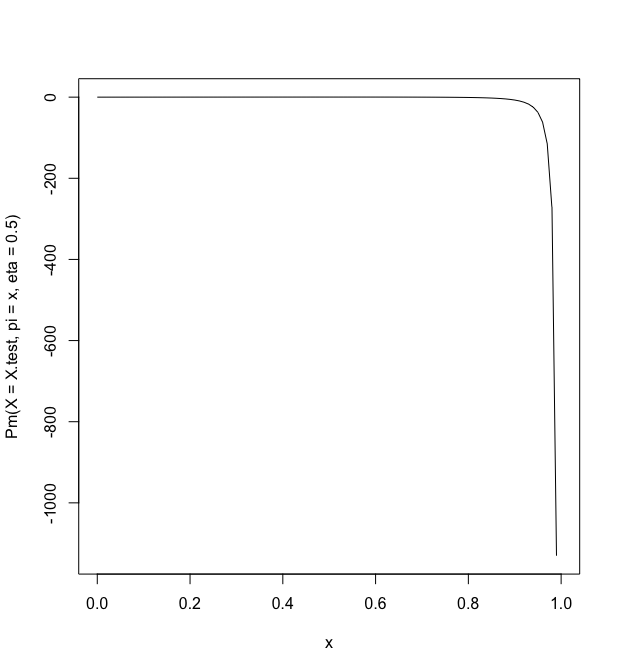
\includegraphics[width=0.5\textwidth]{img/Pm_2.png}
        \caption{À droite: Histogramme d'un échantillon de loi de mélange de lois uniformes de taille $10^3$ avec $\eta^\star=0.5$ et $\pi^\star=0.5$. À gauche: Graphe de la fonction $\pi\mapsto{}P_\mathbb{X}\,m_{\pi,\eta}$ pour un échantillon de loi uniforme sur $\overline{(0,1)}$ de taille $10^3$ avec $\eta=\eta^\star=0.5$ ($\pi^\star=0.5$).}
    \end{figure}

    \begin{figure}[H]
        \centering
        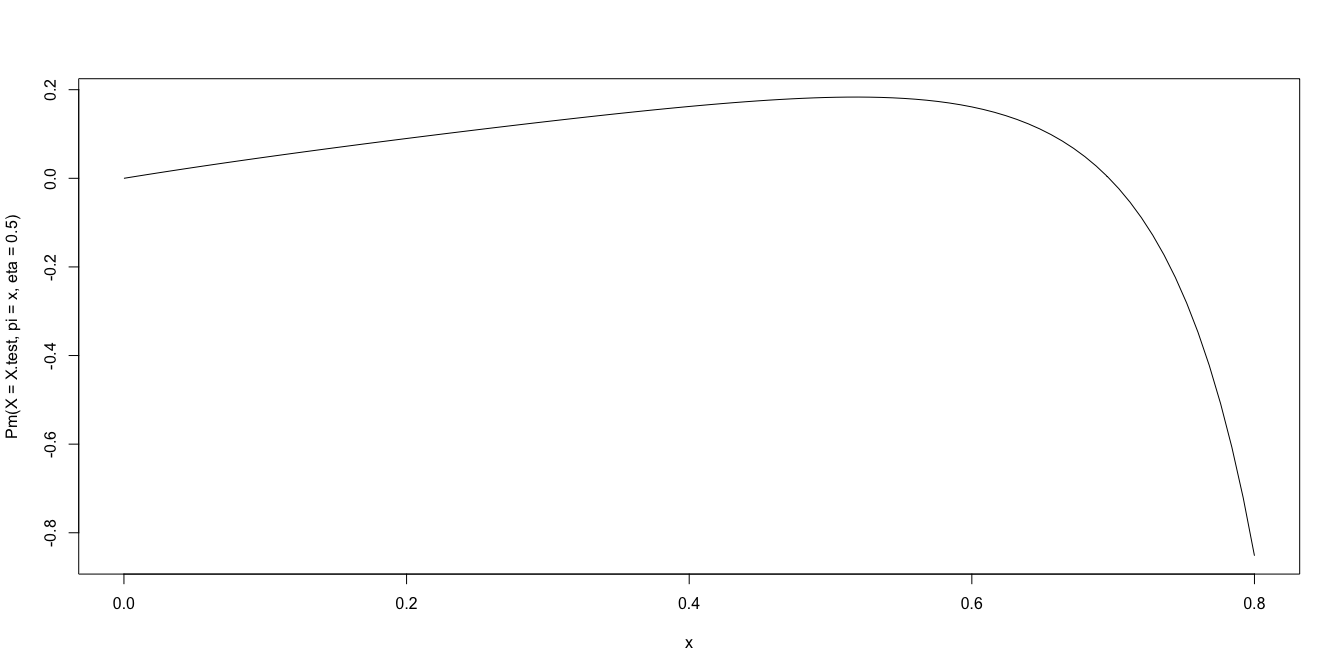
\includegraphics[width=\textwidth]{img/zoom_1.png}
        \caption{Zoom sur le graphe de la fonction $\pi\mapsto{}P_\mathbb{X}\,m_{\pi,\eta}$ pour un échantillon de loi uniforme sur $\overline{(0,1)}$ de taille $10^3$ avec $\eta^\star=\eta=0.5$ ($\pi^\star=0.5$).}
    \end{figure}

    \begin{figure}[H]
        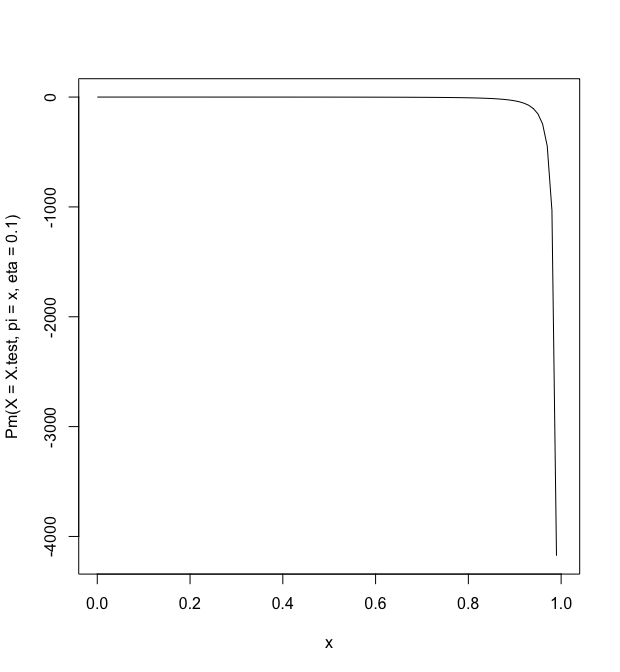
\includegraphics[width=0.475\textwidth]{img/Pm_3.png}
        \hspace{\fill}
        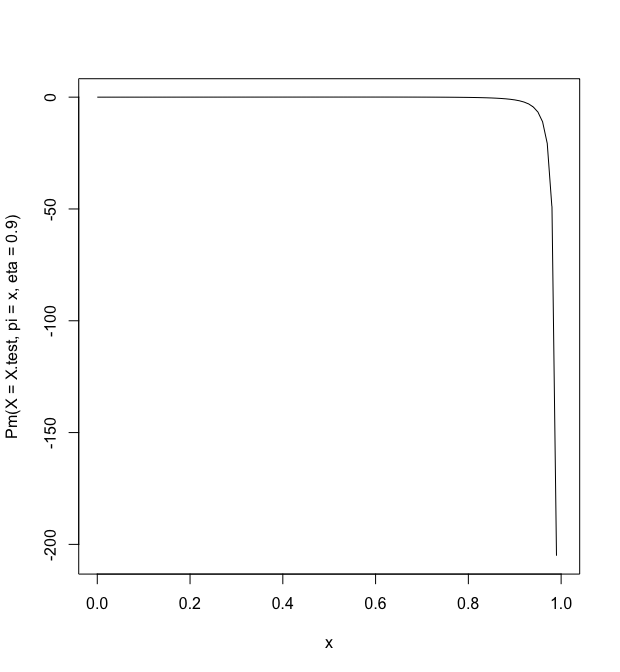
\includegraphics[width=0.475\textwidth]{img/Pm_3bis.png}
        \caption{Graphes de la fonction $\pi\mapsto{}P_\mathbb{X}\,m_{\pi,\eta}$ pour un échantillon de loi uniforme sur $\overline{(0,1)}$ de taille $10^3$ avec $\eta=0.1$ à gauche et $\eta=0.9$ à droite ($\pi^\star=0.5,\,\eta^\star=0.5$).}
    \end{figure}

    \begin{figure}[H]
        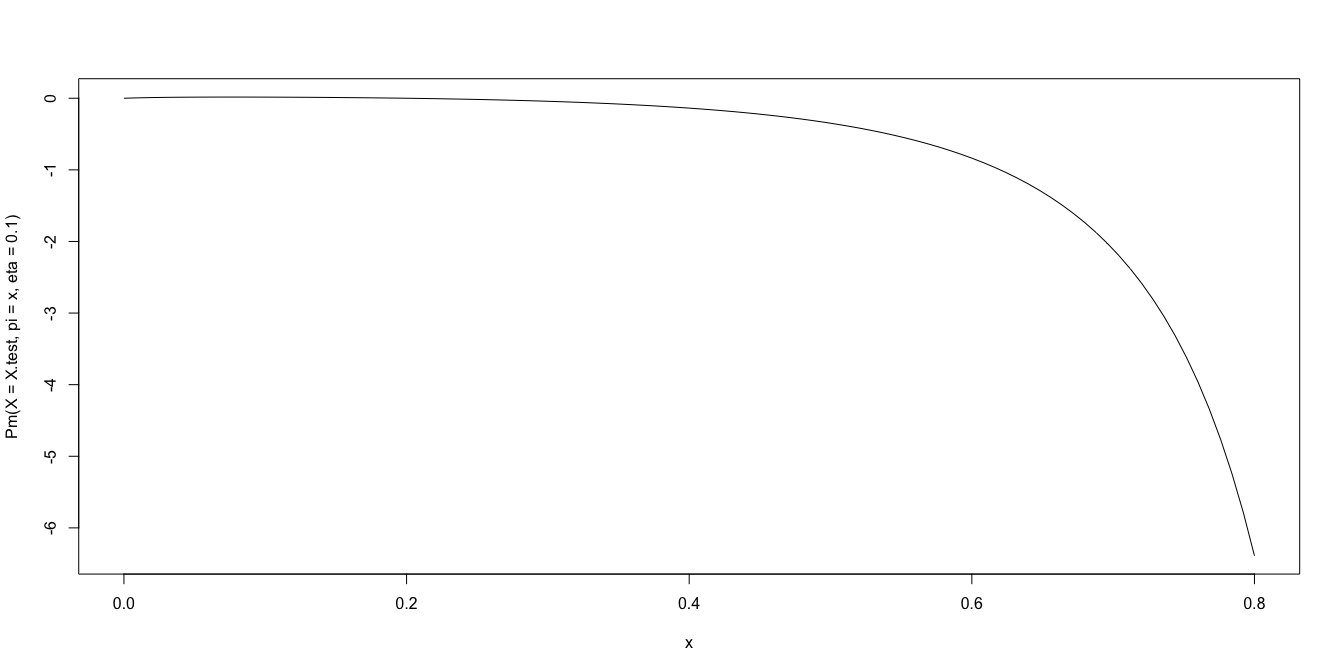
\includegraphics[width=0.475\textwidth]{img/zoom_2.png}
        \hspace{\fill}
        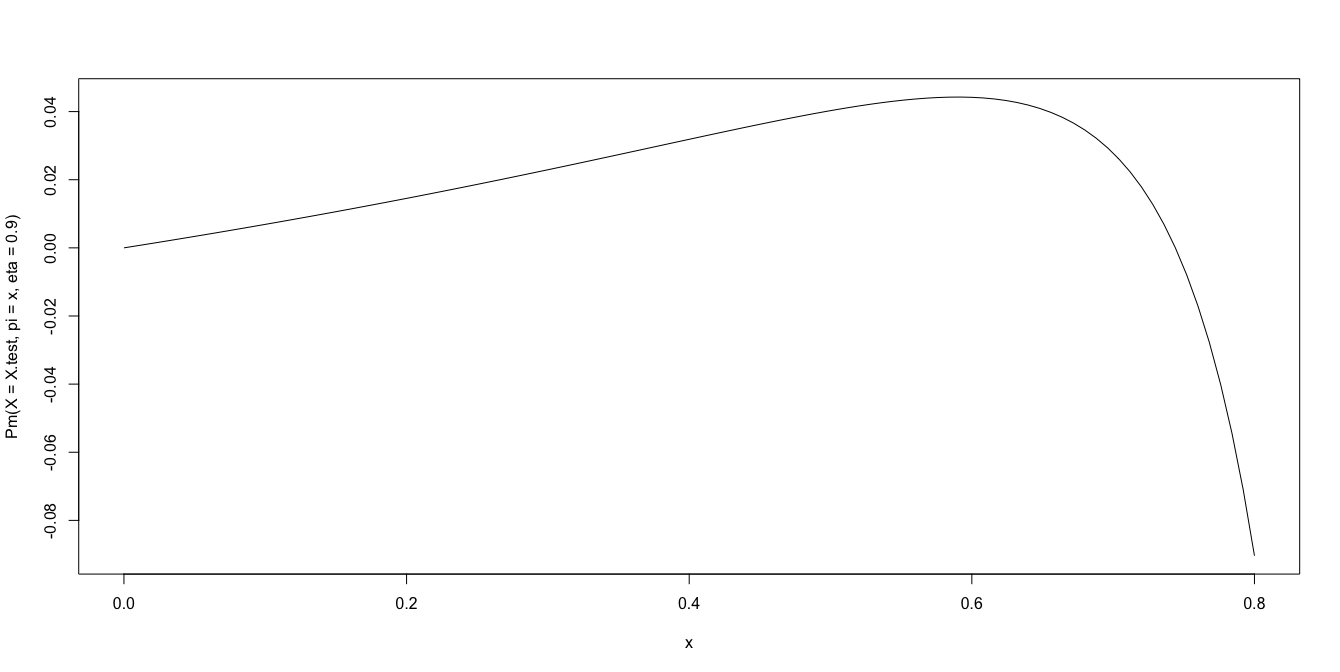
\includegraphics[width=0.475\textwidth]{img/zoom_3.png}
        \caption{Zoom sur les graphes de la fonction $\pi\mapsto{}P_\mathbb{X}\,m_{\pi,\eta}$ pour un échantillon de loi uniforme sur $\overline{(0,1)}$ de taille $10^3$ avec $\eta=0.1$ à gauche et $\eta=0.9$ à droite ($\pi^\star=0.5,\,\eta^\star=0.5$).}
    \end{figure}

    {\color{red} Refaire avec une valeur de $\eta^\star$ différente de $\pi^\star$ pour éviter la confusion.} \\

    Tentons de démontrer la convexité de cette fonction par la positivité de sa dérivée seconde. Appliquons la formule trouvée précédmment au modèle de mélanges de lois uniformes. 

    \begin{align*}
        \partial^2_\pi\,m_{\pi,\eta}(x)   & = 2\cdot\mathop{\mathlarger{\int}}\dfrac{\big[\mathbb{1}_{\overline{(0,1)}}(t)-\frac{1}{\eta}\cdot\mathbb{1}_{\overline{(0,\eta)}}(t)\big]^2}{\{g_{\pi,\eta}(t)\}^3}\cdot\mathrm{d}t - 3\cdot\dfrac{\big[\mathbb{1}_{\overline{(0,1)}}(x)-\frac{1}{\eta}\cdot\mathbb{1}_{\overline{(0,\eta)}}(x)\big]^2}{\{g_{\pi,\eta}(x)\}^4} \\
                                            & = 2\cdot\Big[ \dfrac{\eta\cdot\{1-1/\eta\}^2}{\{1+\dfrac{1-\eta}{\eta}\cdot\pi\}^3} + \dfrac{1-\eta}{\{1-\pi\}^3}\Big] - 3\cdot\Big[ \dfrac{\{1-1/\eta\}^2}{\{1+\dfrac{1-\eta}{\eta}\cdot\pi\}^4}\cdot\mathbb{1}_{\overline{(0,\eta)}}(x) + \dfrac{1}{\{1-\pi\}^4}\cdot\mathbb{1}_{(\eta,1]}(x) \Big]
    \end{align*}

    {\color{red} Peut-on prouver que cette fonction est strictement positive, quel que soient $x$, $\pi$ et $\eta$ ?}

    \subsubsection{Calcul des $a_n$ et $b_n$}

    \begin{align*}
        a(\mathbb{X,\eta})          %&:= \dfrac{P_\mathbb{X}\,\Psi^2_{\hat\pi}}{H_n^2} \\
                                    & := P_\mathbb{X}\big\{ (\partial_\pi\,m_{\hat\pi,\eta})^2 \big\} \Big\backslash \big[ \partial^2_\pi\,P_\mathbb{X}\,m_{\hat\pi,\eta} \big]^2 \\
        \mbox{et, }\quad b_n(\eta,\eta') & := \dfrac{ P_\mathbb{X}\Big[ \partial_\pi\,m_{\hat\pi(\eta),\eta} \cdot \partial_\pi\,m_{\hat\pi(\eta'),\eta'}\Big]}{P_\mathbb{X}\Big[ \partial^2_{\pi}\,m_{\hat\pi(\eta),\eta}\Big] \cdot P_\mathbb{X}\Big[ \partial^2_{\pi}\,m_{\hat\pi(\eta'),\eta'}\Big]}
    \end{align*}

    D'après ce qu'il précède,

    $$ \partial_\pi\, m_{\pi,\eta}(x) = \dfrac{\eta\cdot\{1-1/\eta\} }{\{1+\dfrac{1-\eta}{\eta}\cdot\pi\}^2} + \dfrac{1-\eta}{\{1-\pi\}^2 } - \Big[ \dfrac{1-1/\eta}{\{1+\dfrac{1-\eta}{\eta}\pi\}^3 }\cdot\mathbb{1}_{\overline{(0,\eta)}}(x) + \dfrac{1}{\{1-\pi\}^3}\cdot\mathbb{1}_{(\eta,1]} \Big]  $$

    On s'arrêtre là pour la computation$\backslash$encodage de la fonction $P_\mathbb{X}\{\,(\partial_\pi\,m_{\pi,\eta})^2\}$. \\

    En revanche, du fait que l'on puisse écrire $\partial^2_\pi\,P_\mathbb{X}\,m_{\hat\pi,\eta}  = P_\mathbb{X}\,\partial^2_\pi\,m_{\hat\pi,\eta}$, il vient,

    $$ \partial^2_\pi\,P_\mathbb{X}\,m_{\hat\pi,\eta} =  2\cdot\Big[ \dfrac{\eta\cdot\{1-1/\eta\}^2}{\{1+\dfrac{1-\eta}{\eta}\cdot\hat\pi\}^3} + \dfrac{1-\eta}{\{1-\hat\pi\}^3}\Big] - 3\cdot\Big[ \dfrac{\{1-1/\eta\}^2}{\{1+\dfrac{1-\eta}{\eta}\cdot\hat\pi\}^4}\cdot{}p_- + \dfrac{1}{\{1-\hat\pi\}^4}\cdot{}p_+ \Big]$$ 

    \newpage
    \section{Encodage de l'algorithme}

    \SetKw{Apriori}{Données a priori:}
    \begin{algorithm}[h!]
    \caption{Algorithme général: Test d'homogénéité}
        \Apriori $\phi$, $\{f_1\}$, $\{f_2\}$, $\theta_1^\star$ \\
        \vspace*{0.2cm}
        \textbf{Input:} $n$, $n_{exp}$, $\tilde{n}$, $\mathcal{D}(\Theta_2)$, $\tilde{\mathcal{D}}(\Theta_2)$, $p$ \\
        \begin{enumerate}
            \item Générer le plan d'échantillonnage $\mathbb{X}_{n_{exp},n} = 
            \begin{bmatrix}
                \mathbb{X}^{(1)} \\
                \mathbb{X}^{(2)} \\
                \ldots \\
                \mathbb{X}^{(n_{exp})}
            \end{bmatrix} =
            \begin{bmatrix}
                X_{1,1} & X_{1,2} & \ldots & X_{1,n} \\
                X_{2,1} & X_{2,2} & \ldots & X_{2,n} \\
                \vdots  & \vdots  & \ddots & \vdots  \\
                X_{n_{exp},1} & X_{n_{exp},2} & \ldots & X_{n_{exp},n}
            \end{bmatrix}$ 
            où $X_{i,j} \sim g_{\pi^\star,\theta^\star}$. \hfill \break       
            \item Générer le vecteur $(t_k)_{1\leq k\leq n_{exp}}$ où $t_k := \textrm{Max}_{\eta\in\mathcal{D}(\Theta_2)}\, s_k(\eta)$ avec $s_k(\eta) := s(\mathbb{X}^{(k)},\eta)$. \vspace*{0.2cm}
            \item Générer la matrice $[t_{k,\tilde{k}}]_{\substack{1\leq k\leq n_{exp} \\ 1\leq\tilde{k}\leq\tilde{n}}}$ où $t_{k,\tilde{k}}:=\mathrm{Max}_{\eta\in\tilde{\mathcal{D}}(\Theta_2)}\,Y_\eta(\mathbb{X}^{(k)})$
        \end{enumerate}
        \begin{flushright}
            avec $(Y_\eta(\mathbb{X}))_{\eta\in\tilde{\mathcal{D}}(\Theta_2)}\sim\mathcal{N}(0,\Sigma(\mathbb{X}))$ et $\Sigma(\mathbb{X}):=\Big[\dfrac{b(\mathbb{X,\eta,\eta^\prime})}{\sqrt{a(\mathbb{X},\eta)\cdot{}a(\mathbb{X},\eta^\prime)}}\Big]_{\eta,\eta^\prime\in\tilde{\mathcal{D}}(\Theta_2)}$
        \end{flushright}
        \begin{enumerate}
        \setcounter{enumi}{4}
            \item Calculer le vecteur des probabilités de rejet $r:=\dfrac{1}{n_{exp}}\cdot\sum_{k=1}^{n_{exp}}\mathbb{1}\{t_k\geq t_{k,(\lceil \tilde{n}\cdot (1-p) \rceil)}\}$
        \end{enumerate}
    \end{algorithm}
    avec,
    \begin{align*}
        \hat\pi(\mathbb{X},\eta)    & := \arg\max_\pi\,P_\mathbb{X}\,m_{\pi,\eta} \\
        a(\mathbb{X,\eta})          %&:= \dfrac{P_\mathbb{X}\,\Psi^2_{\hat\pi}}{H_n^2} \\
                                    & := P_\mathbb{X}\big\{ (\partial_\pi\,m_{\hat\pi,\eta})^2 \big\} \Big\backslash \big[ \partial^2_\pi\,P_\mathbb{X}\,m_{\hat\pi,\eta} \big]^2 \\
        s(\mathbb{X},\eta)          & := \sqrt{\dfrac{|\mathbb{X}|}{a(\mathbb{X},\eta)}}\cdot\hat\pi(\mathbb{X},\eta) \\
        \mbox{et, }\quad b_n(\eta,\eta') & := \dfrac{ P_\mathbb{X}\Big[ \partial_\pi\,m_{\hat\pi(\eta),\eta} \cdot \partial_\pi\,m_{\hat\pi(\eta'),\eta'}\Big]}{P_\mathbb{X}\Big[ \partial^2_{\pi\pi}\,mm_{\hat\pi(\eta),\eta}\Big] \cdot P_\mathbb{X}\Big[ \partial^2_{\pi\pi}\,m_{\hat\pi(\eta'),\eta'}\Big]}
    \end{align*}
    \vspace*{0.5cm}

    \newpage
    \subsection{Étape préliminaire: la spécification du mélange}

    \begin{fonction}[h!]
        \caption{Spécification du modèle de mélange \textrm{`\textbf{spec}'} }
             % \Apriori $\{f_1\}$, $\{f_2\}$, $\theta_1^\star$ \\
             % \vspace*{0.2cm}
             \textbf{Arguments:} \texttt{nomDistribution.1, nomDistribution.2, parametrage.1} \\
             \textit{optionnels:} \texttt{nombreParametres.distribution\_2, positionParam.2\_inconnu, \hspace*{1.55cm} valeurParam.2\_connue}
             \begin{itemize}
                 \item[$\bullet$] \texttt{nomDistribution.1, nomDistribution.2}: sont les noms des distributions des composantes du mélanges.
                 Elles sont de types \textit{string}. \\ Les valeurs admises sont: \texttt{"exp", "norm", "lnorm", "weibull","unif"}. \\
                 \vspace*{0.2cm}
                 Exemple: \texttt{nomDistribution.1 = "unif", nomDistribution.2 = "unif"} \\
                 \vspace*{0.2cm}
                 \item[$\bullet$] \texttt{parametrage.1}: est le paramétrage (supposé connu) de la premmière composante. \\
                 \vspace*{0.2cm}
                 Exemples:\begin{itemize}
                     \item[] \texttt{nomDistribution.1 = "norm", parametrage.1 = c(0,1)} pour une loi normale centrée réduite.
                     \item[] \texttt{nomDistribution.1 = "unif", parametrage.1 = c(-1,1)} pour une loi uniforme \\ sur $[-1,1]$. 
                     \item[] \texttt{nomDistribution.1 = "exp", parametrage.1 = 0.5} pour une loi exponentielle de moyenne 2.
                         \end{itemize}
                 \vspace*{0.2cm}
                 \item[$\bullet$] \texttt{nombreParametres.distribution\_2}: est le nombre de paramètre de la seconde composante (sa valeur par défaut vaut 1.) \\
                 \vspace*{0.2cm}
                 Exemples: \texttt{nomDistribution.2 = "norm", nombreParametres.distribution\_2 = 2}
                 \vspace*{0.2cm}
                 \item[$\bullet$] \texttt{positionParam.2\_inconnu}: est la position du paramètre inconnu invernant dans la définition des loi sous R (sa valeur par défaut vaut 1.) \\
                 \vspace*{0.2cm}
                 Exemples: 
                     \begin{itemize}
                         \item[] \texttt{nomDistribution.1 = "norm", positionParam.2\_inconnu = 1} si la moyenne est inconnue. 
                         \item[] \texttt{nomDistribution.1 = "norm", positionParam.2\_inconnu = 1} si c'est l'écart-type qui n'est pas connu. 
                     \end{itemize}
                 \vspace*{0.2cm}
                 \item[$\bullet$] \texttt{valeurParam.2\_connue}: valeur du paramètre connue de la seconde composante (sa valeur par défaut est \texttt{NaN}.)
             \end{itemize}
     \end{fonction}
     \textbf{N.B.}: Les arguments optionnels sont nécessaires si et seulement si la seconde composante admet deux paramètres.
\newpage
     \begin{script}[h!]
         \caption{Spécification du mélange}
         \begin{minted}[linenos, breaklines, fontsize=\scriptsize, bgcolor=lightgray]{R}
             specificationDuMelange = function(nomDistribution.1, 
                                               nomDistribution.2, 
                                               parametrage.1, 
                                               nombreParametres.distribution_2 = 1,
                                               positionParam.2_inconnu = 1,
                                               valeurParam.2_connue = NaN){
 
                 distributionList = c("exp", "norm", "lnorm", "weibull","unif")
                 test = (nomDistribution.1 %in% distributionList) & (nomDistribution.1 %in% distributionList)
                 if( test == FALSE ){ print("Erreur de saisie dans le nom d'une des composantes")}
 
                 # PREMIERE COMPOSANTE # 
                 if(length(parametrage.1) == 1){
                     rf1 = function(n) get(paste0("r", nomDistribution.1))(n, parametrage.1) 
                     df1 = function(x) get(paste0("d", nomDistribution.1))(x, parametrage.1)
                 }
                 if(length(parametrage.1) == 2){
                     rf1 = function(n) get(paste0("r", nomDistribution.1))(n, parametrage.1[1], parametrage.1[2])
                     df1 = function(x) get(paste0("d", nomDistribution.1))(x, parametrage.1[1], parametrage.1[2])
                 }
                 assign("rf1", rf1, envir = .GlobalEnv)
                 assign("df1", df1, envir = .GlobalEnv)
 
                 # DEUXIEME COMPOSANTE #
                 if(nombreParametres.distribution_2 == 1){
                     rf2 = function(n,eta) get(paste0("r", nomDistribution.2))(n, eta)
                     df2 = function(x,eta) get(paste0("d", nomDistribution.2))(x, eta)
                 }
                 else{ # nombreParametres.distribution_2 == 2
                 if(nombreParametres.distribution_2 != 2) return("Erreur: Le nombre de paramètres de la composante ne peut que prendre les valeurs 1 ou 2.")
                 if(positionParam.2_inconnu == 1){
                     rf2 = function(n,eta) get(paste0("r", nomDistribution.2))(n, eta, valeurParam.2_connue)
                     df2 = function(x,eta) get(paste0("d", nomDistribution.2))(x, eta, valeurParam.2_connue)
                 }
                 else{ # positionParam.2_inconnu == 2
                 if(positionParam.2_inconnu != 2) return("Erreur: La position du paramètre inconnu de la seconde composante.")
                     rf2 = function(n,eta) get(paste0("r", nomDistribution.2))(n, valeurParam.2_connue, eta)
                     df2 = function(x,eta) get(paste0("d", nomDistribution.2))(x, valeurParam.2_connue, eta)
                 }
                 }
                 assign("rf2", rf2, envir = .GlobalEnv)
                 assign("df2", df2, envir = .GlobalEnv)
 
                 # FONCTIONS DU MELANGE #
                 rmix = function(n,pi,eta){
                     output = sample(x = c(0,1), size = n, replace = TRUE, prob = c(1-pi,pi))
                     
                     nb1 = sum(output)
                     
                     output[output == 1] = rf2(nb1,eta)
                     output[output == 0] = rf1(n-nb1)
                     
                     return(output)
                 }
                 dmix = function(x,pi,eta) (1-pi)*df1(x) + pi*df2(x,eta)
 
                 assign("rmix", rmix, envir = .GlobalEnv)
                 assign("dmix", dmix, envir = .GlobalEnv)
             }
         \end{minted}
     \end{script}
 
\newpage
    \subsection{Première étape}


    $$ \mbox{Générer le plan d'échantillonnage } \mathbb{X}_{n_{exp},n} = 
    \begin{bmatrix}
        \mathbb{X}^{(1)} \\
        \mathbb{X}^{(2)} \\
        \ldots \\
        \mathbb{X}^{(n_{exp})}
    \end{bmatrix} =
    \begin{bmatrix}
        X_{1,1} & X_{1,2} & \ldots & X_{1,n} \\
        X_{2,1} & X_{2,2} & \ldots & X_{2,n} \\
        \vdots  & \vdots  & \ddots & \vdots  \\
        X_{n_{exp},1} & X_{n_{exp},2} & \ldots & X_{n_{exp},n}
    \end{bmatrix}$$

    \begin{fonction}
        \caption{Génération du plan d'échantillonnage \texttt{MATRICE\_ECHANTILLONAGE}}
        \Apriori Spécification du mélange via la fonction \texttt{SPECIFICATIION\_DU\_MELANGE}. \\
        \vspace*{0.2cm}
        \textbf{Arguments:} \texttt{nexp, n, pi.star, eta.star}
        \begin{itemize}
            \item[$\bullet$] \texttt{nexp}: nombre d'échantillon à générer.
            \item[$\bullet$] \texttt{n}: taille des échantillons.
        \end{itemize}
        \vspace*{0.2cm}
        \textbf{Définit lors de l'execution}: Dans l'environnement global ($i.e.$: \texttt{.GlobalEnv}) la matrice \texttt{matrice.dechantillonnage} de taille ($n_{exp}\times{}n$) où pour tout $i,j$: $\quad\mathbf{x}_{i,j}\sim{}g_{\pi^\star,\theta^\star}$.
    \end{fonction}
    \begin{script}[h]
        \begin{minted}[linenos, breaklines, fontsize=\scriptsize, bgcolor=lightgray]{R}
            MATRICE_ECHANTILLONNAGE = function(nexp, n, pi.star, eta.star){
                if(!exists("rmix")) "La spécification du mélange n'a pas opérée."
  
                matrice.dechantillonnage = matrix(data = rmix(n = n*nexp, pi = pi.star, eta = eta.star), nrow = nexp, byrow = TRUE)
                assign("matrice.dechantillonnage", matrice.dechantillonnage, envir = .GlobalEnv)
            }
        \end{minted}
    \caption{Génération de la matrice d'échantillonnage}
    \end{script}

    \newpage

    \subsection{Deuxième étape: }

    $$ \mbox{Générer le vecteur } (t_k)_{1\leq k\leq n_{exp}} \mbox{ où } t_k := \textrm{Max}_{\eta\in\mathcal{D}(\Theta_2)}\, s_k(\eta) \mbox{ avec } s_k(\eta) := s(\mathbb{X}^{(k)},\eta) = \sqrt{\dfrac{|\mathbb{X}|}{a(\mathbb{X}^{(k)},\eta)}}\cdot\hat\pi(\mathbb{X}^{(k)},\eta)$$


    \subsubsection{Encodage des sous-fonctions}
    \begin{fonction}
        \caption{Sous-fonction \texttt{CALCUL\_STATISTIQUE} $\backslash\backslash$ Mélanges Uniformes dans le cas $\chi^2$}
        \Apriori $\mathbb{X}(\omega)=\mathbf{x}$ \\
        \vspace*{0.2cm}
        \textbf{Arguments:} \texttt{echantillon, eta}
        \begin{itemize}
            \item[$\bullet$] \texttt{echantillon}: le vecteur des données $\mathbf{x}$.
            \item[$\bullet$] \texttt{eta}: le paramètre $\eta$ sous lequel les calculs sont effectués. 
        \end{itemize}
        \textbf{Sortie:} \texttt{hatpi, an, s}
        \begin{itemize}
            \item[$\bullet$] \texttt{hatpi}: il s'agit de $\hat\pi(\mathbf{x},\eta)$ ;
            \item[$\bullet$] \texttt{an}: correspond à $a(\mathbf{x},\eta)$ ;
            \item[$\bullet$] \texttt{s}: renvoie à $s(\mathbf{x},\eta)$.   
        \end{itemize}
    \end{fonction}


    \begin{script}
        \caption{Calcul des statistques}
        \begin{minted}[linenos, breaklines, fontsize=\scriptsize, bgcolor=lightgray]{R}

            Pm = function(echantillon, pi, eta){
                a = 1 + pi*(1/eta-1)
                b = 1 - pi
                
                n.moins = sum(echantillon<eta)
                n = length(echantillon)
                n.plus = n - n.moins
                
                A = (b*eta + a*(1-eta))/(a*b)
                B = 0.5*(1+(n.moins/a**2 + n.plus/b**2)/n)
                
                output = A - B
                return(output)
              }
              
              partial.pi_m = function(pi,eta,x){
                premier.terme = eta*(1-1/eta)/(1+(1-eta)*pi/eta)**2 + (1-eta)/(1-pi)**2
                
                if(x < eta) second.membre = (1-1/eta)/(1+(1-eta)*pi/eta)**3
                else second.membre = 1/(1-pi)**3
              
                return(premier.terme - second.membre)
              }
              
              partial.pi_m__SQUARRED = function(pi,eta,x) partial.pi_m(pi,eta,x)**2
              
              partial2.pi_Pm = function(pi,eta,echantillon){
                n = length(echantillon)
                n.moins = sum(echantillon < eta)
                p.moins = sum(echantillon < eta)/n
                p.plus = (n - n.moins)/n
                
                premier.terme = 2*( eta*(1-1/eta)**2/(1+(1-eta)*pi/eta)**3 + (1-eta)/(1-pi)**3 )
                second.terme = 3*( p.moins*(1-1/eta)**2/(1+(1-eta)*pi/eta)**4 + p.plus/(1-pi)**4  ) 
                
                return(premier.terme - second.terme)
              }
              
              HATPI = function(echantillon, eta){
                temp.fun = function(pi) Pm(echantillon = echantillon, pi = pi, eta = eta)
                return(optimise(f = temp.fun, interval = c(0,1), maximum = TRUE)$maximum)
              } 
              
              AN = function(echantillon,hatpi,eta){
                
                numerateur = mean(sapply(echantillon, partial.pi_m__SQUARRED, pi = hatpi, eta = eta))
                denominateur = partial2.pi_Pm(pi = hatpi, eta = eta, echantillon = echantillon)**2
                
                
                return(numerateur/denominateur)
              }
              
              
              
              
              CALCUL_STATISTIQUE = function(echantillon, eta){
                n = length(echantillon)
              
                hatpi = HATPI(echantillon = echantillon, eta = eta)
                an = AN(echantillon = echantillon, hatpi = hatpi, eta = eta)
              
                sn = sqrt(n/an)*hatpi
              
              #  return(data.frame(hatpi,an,s))
                return(c(hatpi,an,sn))
              }
              

            }
            
        \end{minted}
    \end{script}

    \begin{center}
        $ (\mathbb{X},\eta) \longmapsto (\hat\pi(\mathbb{X},\eta),a(\mathbb{X},\eta),s(\mathbb{X},\eta)) $
    \end{center}


    \begin{fonction}[h]
        \caption{\texttt{MATRICE\_STATISTIQUE}}
        \textbf{Arguments:} \texttt{matrice.dechantillonnage, eta} \\
         \texttt{matrice.dechantillonnage}: $\mathbb{X}_{n_{exp},n}$ \\
         \texttt{eta}: $\eta$ \\
         \textbf{Définit lors de l'execution:} Dans l'environnement global ($i.e.$: \texttt{.GlobalEnv}) la matrice \texttt{matrice.statistique}.
     \end{fonction}
 
     \begin{script}[t]
         \caption{Matrice de statistiques}
         \begin{minted}[linenos, breaklines, fontsize=\scriptsize, bgcolor=lightgray]{R}
             MATRICE_STATISTIQUE = function(matrice.dechantillonnage, eta){
                 matrice.statistique = t(apply(X = matrice.dechantillonnage, eta = eta, FUN = CALCUL_STATISTIQUE, MARGIN = 1))
                 
                 matrice.statistique = data.frame(matrice.statistique)
                 names(matrice.statistique) = c("hatpi","an","t")
                 
                 assign("matrice.statistique", matrice.statistique, envir = .GlobalEnv) 
               }
         \end{minted}
     \end{script}
 
 
     $$
     (\mathbb{X}_{n_{exp},n}, \eta) =                         
     (\begin{bmatrix}
         \mathbb{X}^{(1)} \\
         \mathbb{X}^{(2)} \\
         \ldots \\
         \mathbb{X}^{(n_{exp})}
     \end{bmatrix},\eta) 
     \longmapsto 
     \begin{bmatrix}
         \hat\pi(\mathbb{X}^{(1)},\eta) & a(\mathbb{X}^{(1)},\eta) & s(\mathbb{X}^{(1)},\eta) \\
         \hat\pi(\mathbb{X}^{(2)},\eta) & a(\mathbb{X}^{(2)},\eta) & s(\mathbb{X}^{(2)},\eta) \\
         \vdots & \vdots & \vdots \\
         \hat\pi(\mathbb{X}^{(n_{exp})},\eta) & a(\mathbb{X}^{(n_{exp})},\eta) & s(\mathbb{X}^{(n_{exp})},\eta) \\
     \end{bmatrix}
     $$

    \newpage
    \subsubsection{Encodage du vecteur}

    \begin{fonction}[h]
        \caption{\texttt{VECTEUR\_T}}
    \end{fonction}
    \begin{script}[h]
        \caption{\texttt{VECTEUR\_T}}
        \begin{minted}[linenos, breaklines, fontsize=\scriptsize, bgcolor=lightgray]{R}
            VECTEUR_T = function(matrice.dechantillonnage, discretisation.Theta_2){
                vecteur.s = sapply(X = discretisation.Theta_2, FUN = (function(eta) MATRICE_STATISTIQUE(matrice.dechantillonnage, eta)$s) )
                assign("vecteur.s", vecteur.s, envir = .GlobalEnv)
                vecteur.t = apply(X = vecteur.s, FUN = max, MARGIN = 1)
                assign("vecteur.t", vecteur.t, envir = .GlobalEnv)
            }
        \end{minted}
    \end{script}

    \subsection{Troisième étape}
    \begin{center}
    Générer la matrice $[t_{k,\tilde{k}}]_{\substack{1\leq k\leq n_{exp} \\ 1\leq\tilde{k}\leq\tilde{n}}}$ où $t_{k,\tilde{k}}:=\mathrm{Max}_{\eta\in\tilde{\mathcal{D}}(\Theta_2)}\,Y_\eta(\mathbb{X}^{(k)})$
        \begin{flushright}
            avec $(Y_\eta(\mathbb{X}))_{\eta\in\tilde{\mathcal{D}}(\Theta_2)}\sim\mathcal{N}(0,\Sigma(\mathbb{X}))$ et $\Sigma(\mathbb{X}):=\Big[\dfrac{b(\mathbb{X,\eta,\eta^\prime})}{\sqrt{a(\mathbb{X},\eta)\cdot{}a(\mathbb{X},\eta^\prime)}}\Big]_{\eta,\eta^\prime\in\tilde{\mathcal{D}}(\Theta_2)}$
        \end{flushright}
    \end{center}





































    %%%%%%%%%%%%%%%%%%%%%%%%%%%%%%%%%%%%%%%%%%%%%%%%%%%%%%%%%%%%%%%%%%%%%%%%%%%%%%%%%%%%%%%%%%%%%%%%%%%%%%%%%%%%%%%%%%%%%%%%%%%%%%%%%%%%%%%%%%%%%%%%%%%%%%%%%%%%%%%%%%%%%%%%%%%%%%%%%%%%%%%%    
    %%%%%%%%%%%%%%%%%%%%%%%%%%%%%%%%%%%%%%%%%%%%%%%%%%%%%%%%%%%%%%%%%%%%%%%%%%%%%%%%%%%%%%%%%%%%%%%%%%%%%%%%%%%%%%%%%%%%%%%%%%%%%%%%%%%%%%%%%%%%%%%%%%%%%%%%%%%%%%%%%%%%%%%%%%%%%%%%%%%%%%%%
    
    
    \newpage
    \section{Past work...}


 
    Nous reprenons le même algorithme que précédemment, cette fois appliqué pour la divergence du $\chi^2$. \\

    \section{Etude de l'algorithme dans le cas $\chi^2$}

    \underline{Etape 1}: Générer $\mathbb{X}_{n_{exp},n}$ idem que pour KL$_m$ car indépendante de la divergence. \\

    \underline{Etape 2}: Générer le vecteur $(t_k)_{1\geq k\geq n_{exp}}$. \\

    $$ t_k := \max_{\eta\in\mathcal{D}(\Theta_2)}\, s_k(\eta) \mbox{ avec } s_k(\eta) := \sqrt{\dfrac{|\mathbb{X}|}{a(\mathbb{X},\eta)}}\cdot\hat\pi(\mathbb{X},\eta)$$

    Ici les notions dépendent de la divergence, nous explicitons donc un peu plus en ce sens. \\

    \subsection{Calcul de $\hat\pi$}

    Nous avons toujours: $\hat\pi(\mathbb{X},\eta) = \max_\pi\, P_\mathbb{X}\, m_{\pi,\eta}$ \\

    D'après nos calculs {\color{green} (vérifiée }[OK]{\color{green})} nous avions, pour toute fonction $g$ d'intégrale $1$,
    $$ P_\mathbb{X}\,m_{\pi,\eta} = \dfrac{1}{a\cdot{}b}\Big\{b\cdot\int_0^\eta(g(t))^2\mathrm{d}t + a\cdot\int_\eta^1(g(t))^2\mathrm{d}t\Big\} - \dfrac{1}{2}\Big\{ 1 + \dfrac{1}{n}\Big[ \sum_{x_i\leq\eta} \Big(\dfrac{g(x_i)}{a}\Big)^2 + \sum_{x_i>\eta}\Big(\dfrac{g(x_i)}{b}\Big)^2 \Big]\Big\}$$

    où $a=1+\pi\cdot(\dfrac{1}{\eta}-1)$ et $b=1-\pi$. \\

    En particulier, lorsque nous faisons le choix $g\equiv\mathbb{1}_{\overline{(0,1)}}$,
    $$ P_{\mathbb{X}}\, m_{\pi,\eta} = \dfrac{1}{ab}\Big[ b\cdot\eta + a\cdot(1-\eta)\Big] - \dfrac{1}{2}\Big[ 1 + \dfrac{1}{n}\cdot(\dfrac{n_-}{a^2} + \dfrac{n_+}{b^2})\Big] $$

    où $n_+$ (respectivement $n_-$) est le nombre de données $x_i$ de $\mathbb{X}(\omega)$ supérieures à $\eta$ (respectivement inférieures à $\eta$).\\ 
    
    Nous devons trouver $\hat\pi_n(\eta) := \max_\pi\, P_{\mathbb{X}}\, m_{\pi,\eta}$ si toutefois il existe. \\

    Remarquons alors, que la fonction qui à $\pi$ associe $P_{\mathbb{X}}\, m_{\pi,\eta}$ (comme formulé précédemment) est continue ({\color{red} sauf peut-être en 0}), et cela quel que soit $\eta$. Ainsi dès lors que $\pi$ appartient au compact $\overline{(0,1)}$, cette fonction atteint ses bornes. Prouvant ainsi l'existence d'un tel maxima. \\

    En outre, si nous arrivions à démontrer la convexité de $\pi\longmapsto P_{\mathbb{X}}\,m_{\pi,\eta}$ quel que soit $\eta$. Nous pourrions affirmer qu'il existe un unique maximum $\hat\pi$ à cette fonction. \\

    {\color{green} Malheureusement cela semble assez fastidieux à démontrer lorsque l'on cherche à prouver la positivité stricte de la dérivée seconde. \\
    
    D'après mes calculs, nous serions ramener à dévoir démonter l'inégalité stricte suivante:
    $$ \dfrac{2}{3}\int_0^1\dfrac{\big\{f_1(t)-f_2(t,\eta)\big\}^2}{\Big(g_{\pi,\eta}(t))^3}\mathrm{d}t\,>\,\dfrac{\big\{f_1(t)-f_2(t,\eta)\big\}^2}{\Big(g_{\pi,\eta}(t))^4} $$
    
    Autrement dit, que:

    $$\dfrac{2}{3}\cdot\Big[ \dfrac{\eta(1-1/\eta)^2}{\{1-(1-1/\eta)\pi\}^3} + \dfrac{1-\eta}{(1-\pi)^3} \Big]$$

    est strictement supérieur à: {\color{red} affirmation douteuse... !}

    $$ \dfrac{1}{(1-\pi)^4} \mbox{ et } \dfrac{(1-1/\eta)^2}{(1-(1-1/\eta)\pi)^4} \mbox{ à la fois }$$
    }
    {\color{red} Nous détaillons les calculs amenant ces des dernières affirmations en annexe !} \\


    Il nous faudra discuter de la méthode de maximisation d'une telle fonction ! 

    \subsection{Calcul de $a_n$}

    Par définition:
    \begin{align*}
        a(\mathbb{X,\eta}) :&= \dfrac{P_\mathbb{X}\,\Psi^2_{\hat\pi}}{H_n^2} \\
                            &= P_\mathbb{X}\big\{ (\partial_\pi\,m_{\hat\pi,\eta})^2 \big\} \Big\backslash \big[ \partial^2_\pi\,P_\mathbb{X}\,m_{\hat\pi,\eta} \big]^2
    \end{align*}

    {\color{red}N'ayant pas d'identité de Fisher pour la divergence du $\chi^2$}, la simplification faite à ce moment là dans le cas KL$_m$ n'est plus possible ici. Nous calculons alors directement le numérateur et dénominateur. \\

    Nous sommes à présent en mesure de calculer $a(\mathbb{X},\eta)$ (ou $a_n$). \\

    {\color{red}À ce stade, l'étape 2 de l'algorithme est alors réalisable numériquement.}

    \subsection{Encodage de l'étape 2}
    \subsubsection{Méthode de maximisation - celle de R}
    

    \subsection{Calcul des $b(\eta,\eta^\prime)$}

    $b(\eta,\eta^\prime)$ est le coefficient (1,1) de la matrice,
    $$ \{P_\mathbb{X}\,H_n^t\}^{-1}\cdot\{P_\mathbb{X}\Psi^\eta_n{}\Psi^{\eta^\prime}_n\}\cdot\{P_\mathbb{X}\,H_n^t\}^{-1}$$

    Avec, lorsque $\theta_1^\star$ est supposé connu:
    \begin{align*}
        \Psi^\eta_n &:= \partial_\pi\,m_{\hat\pi,\theta^\star(\eta)} \\
        H^\eta_n &:= \partial^2_\pi\,m_{\hat\pi,\theta^\star(\eta)}
    \end{align*}

    {\color{red} Attention: L'égalité dite de Fisher $\partial^2_{\pi\pi}\,m_{\hat\pi(t),t} = -\{\,\partial\pi\,m_{\hat\pi(t),t}\,\}^2$ n'est vérififée uniquement dans le cas de la divergence KL$_m$} \\

    Ainsi,   $$b_n(t,t^\prime) := \dfrac{ P_\mathbb{X}\Big[ \partial_\pi\,m_{\hat\pi(t),t} \cdot \partial_\pi\,m_{\hat\pi(t'),t'}\Big]}{P_\mathbb{X}\Big[ \partial^2_{\pi\pi}\,mm_{\hat\pi(t),t}\Big] \cdot P_\mathbb{X}\Big[ \partial^2_{\pi\pi}\,m_{\hat\pi(t'),t'}\Big]}$$

\end{document}
